\documentclass{article}

\title{Create your first Chrome extension}
\author{Bastien Boymond}
\date{}

\usepackage[utf8]{inputenc}
\usepackage[T1]{fontenc}
\usepackage{xcolor}
\usepackage{listings}
\usepackage{hyperref}
\usepackage{graphicx}

\graphicspath{ {../images/} }

\begin{document}
    \maketitle
    \begin{center}
        
\includegraphics[scale=0.1]{../images/chromeExtension.png}
    \end{center}
    \newpage
    \begin{description}
        \item[1 :]{C'est quoi une extension Chrome ?} \\\\ \textbf{\href{https://chrome.google.com/webstore/category/extensions?hl=fr&authuser=0}{Chrome Web Store}} est la plate-forme de téléchargement de Google à destination de son navigateur \textbf{\href{https://www.google.com/intl/fr_fr/chrome/}{Google Chrome}} et de son système d'exploitation Google Chrome OS.
        \begin{center} 
            \rule{0.75\linewidth}{1pt}
        \end{center}
        \item[2 :]{Les dépendances}
\begin{lstlisting}[language=sh]
    sudo apt-get update
    sudo apt-get upgrade
    sudo apt-get install nodejs npm
\end{lstlisting}
        \begin{center} 
            \rule{0.75\linewidth}{1pt}
        \end{center}
        \item[3 :]{Créer un projet Chrome Extension}
\begin{lstlisting}[language=sh]
    mkdir chromeExtension
    cd chromeExtension
    npm init
\end{lstlisting}
        Une fois ça fais vous allez devoir Créer un fichier manifest.json et un fichier index.js.
        \\ Votre Manifest.json doit ressembler à ça :
        \begin{center}
            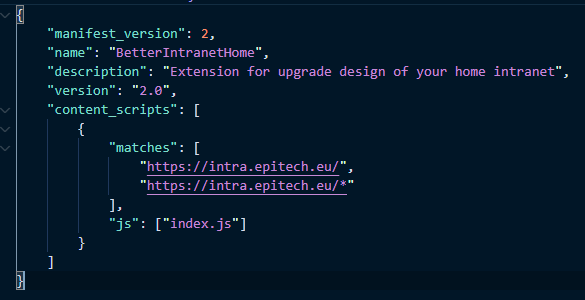
\includegraphics[scale=0.9]{../images/HowToManifest.PNG}
        \end{center}
        Actuellement vous avez fais une extension Chrome qui ne fait rien.
        Cette extension a le droit de toucher a seulement au site de \textbf{\href{https://intra.epitech.eu/}{l'intranet}} C'est donc sur ce site que nous allons faire notre 1ere extension.
        \begin{center}
            \rule{0.75\linewidth}{1pt}
        \end{center}
        \item[4 :]{Tester votre extension Chrome} \\ Vous allez devoir tester votre extension Chrome. Pour cela il vous faut aller sur le site chrome://extensions/
        \\ Passez en mode Développer puis cliquez sur Charger l'extension non empaquetée.
        \begin{center}
            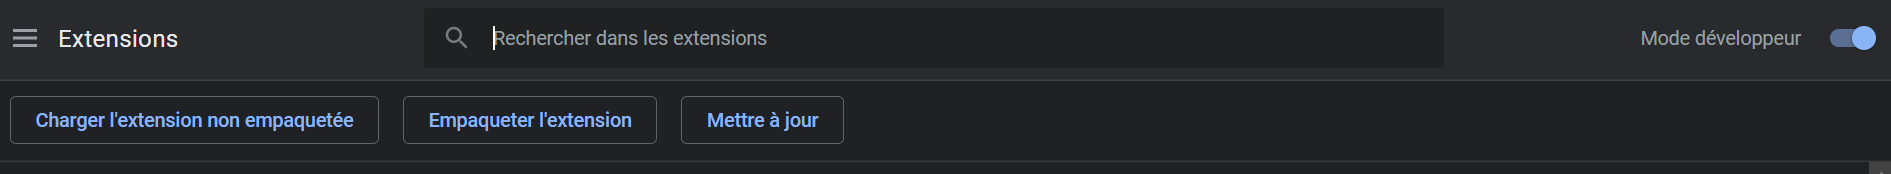
\includegraphics[scale=0.3]{HowToTestChorme.PNG}
        \end{center}
        Vous avez maintenant une extension qui fait rien.
        \begin{center}
            \rule{0.75\linewidth}{1pt}
        \end{center}
        \item[5 :]{Commencer a coder votre extension Chrome} \\ Maintenant que vous avez testé votre extension, vous allez pouvoir commencer a coder votre extension.
        \\ Notre objectif est de créer une extension qui affiche des informations sur la page home de l'intranet.
        \\ Pour cela nous allors cherchez dans l'html de la page home de l'intranet l'endroit si dessous :
        \begin{center}
            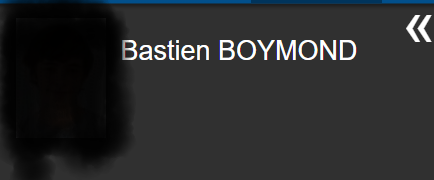
\includegraphics[scale=0.5]{FindInHtml.PNG}
        \end{center}
        Une fois trouver nous allons créer une fonction qui va récupérer l'endroit en html correspondant à l'endroit que nous cherchons.
        \begin{center}
            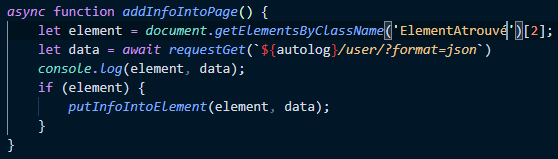
\includegraphics[scale=0.8]{indexjspremierePartie.PNG}
        \end{center}
        La variable element repressente l'endroit que nous cherchons.
        \begin{center}
            \rule{0.75\linewidth}{1pt}
        \end{center}
        \item[6 :]{Récupérer la donner que l'on veux rajouter a notre site} \\ Maintenant que nous avons récupéré l'endroit que nous cherchons nous allons récupérer la donnée que nous cherchons a ajouter a notre site.
        \\ Pour cela nous allons faire une requete avec l'API de l'intranet.
        \begin{center}
            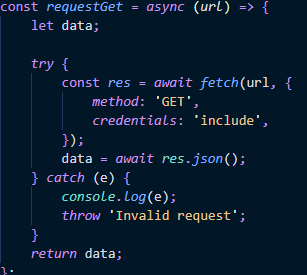
\includegraphics[scale=0.9]{requestGetSansLib.PNG}
        \end{center}
        L'url correspond a votre autologin que vous pouvez trouver a cette url : https://intra.epitech.eu/admin/autolog
        \\ Le lien ressemblera donc a une chose de ce genre : \\ \textbf{https://intra.epitech.eu/auth-f68d1af2174139ebceyvfde5646b4d/user/format=json} (L'autologin ici n'existe pas)
        \begin{center}
            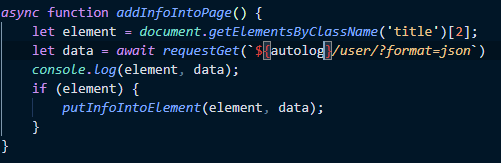
\includegraphics[scale=0.8]{indexjsdeuxiemepartie.PNG}
        \end{center}
        Maintenant que nous avons récupérer la donnée il est tant de la rajouter a notre site.
        \begin{center}
            \rule{0.75\linewidth}{1pt}
        \end{center}
        \item[7 :]{Rajouter la donnée a notre site} \\ Maintenant que nous avons toute les information dont nous avons besoin nous allons rajouter la donnée a notre site.
        \\ Nous allons donc toucher a la fonction putInfoIntoElement Crée plus tot.
        \\ Les taches a faire :
        \begin{itemize}
            \item Supprimer l'element <br>
            \item trouver dans data ton Gpa t'es Crédits et t'as promotion
            \item Ajouter la donnée dans l'element
        \end{itemize}
        Une fois fait le resultat doit ressembler a ça :
        \begin{center}
            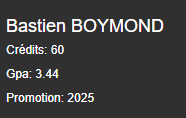
\includegraphics[scale=0.8]{final.PNG}
        \end{center}
        \item[8 :]{Pour allez plus loin} \\ Maintenant que nous avons rajouté la donnée a notre site nous allons pouvoir faire plus de choses.
        \\ Je vais vous proposer plusieur chose a faire pour allez plus loin :
        \begin{itemize}
            \item Crée une popup qui affiche des information d'epitech
            \item Mettre une image a votre extension
            \item Ajouter un bouton a votre extension qui vous inscrit a des projet
            \item rendre le site web plus attractif
        \end{itemize}
    \end{description}
\end{document}